\documentclass[12pt,a4paper,titlepage]{report}
\usepackage[utf8]{inputenc}
\usepackage[portuguese]{babel}
\usepackage[T1]{fontenc}
\usepackage{amsmath}
\usepackage{amsfonts}
\usepackage{amssymb}
\usepackage{makeidx}
\usepackage{graphicx}
\usepackage{lmodern}
\usepackage{wrapfig}
\usepackage{color}
\usepackage{float}
%\usepackage{fourier}
\usepackage[left=2cm,right=2cm,top=2cm,bottom=2cm]{geometry}
\author{Bartolomeu J. Ubisse}
\begin{document}


\begin{figure}[htb]

\centering

\includegraphics[scale=1]{UEM-logotipo}
\end{figure}
\centering
{ \Large Universidade Eduardo Mondlane}\\[0.5cm] 
\large Faculdade de Ci\^encias\\[0.2cm]
 \large Departamento de F\'isica\\[1cm]

\textsc{Electr\^onica B\'asica} \\[1cm]
\begin{flushleft}
2017-AP\# 1-Princ\'ipios b\'asicos de an\'alise de circu\'itos el\'ectricos - Key Answer\\
\hrulefill
\end{flushleft}
\begin{enumerate}
\item Explique o que entende por elementos passivos e dê exemplo de pelo menos quatro deles.\\ \color{red} \textit{- Elementos passivos s\~ao todos aqueles que n\~ao geram energia mas sim dessipam (eg.resistores) assim como armazenam(eg.capacitores e indutores).}\color{black}
\item Se a resistência de um fio de cobre a $25^o$c é $25\Omega$  , determine a sua resistência a uma temperatura de $100^o$c e o seu coeficiente de temperatura. (Considere a temperatura absoluta inferida de Cobre de $-234,5^o$c)\\ 

\begin{figure}[h]
\centering
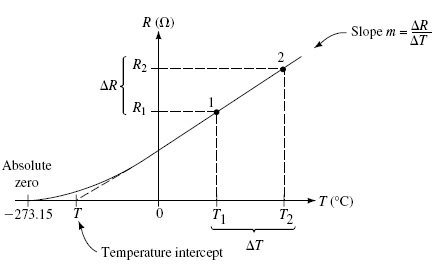
\includegraphics[scale=0.7]{TEffect}
\end{figure}
\small
\color{red}
\begin{eqnarray}
\frac{R_1}{T_1-T}=\frac{R_2}{T_2-T}\Longrightarrow R_2=\frac{T_2-T}{T_1-T}\\ R_2=\frac{100+234.5}{25+234.5}\times 54\Omega =69.6\Omega \\
\alpha=\frac{R_2-R_1}{(T_2-T_1)R_1}=0.00385(^oC)^{-1}
\end{eqnarray}
\vspace{1cm}
\color{black}
\normalsize
\item Explique porque quando se aumenta a temperatura de um certo condutor ele tende a oferecer maior resistência à passagem de corrente eléctrica.\\
\color{red}\textit{- Quando a temperatura \'e maior a vibra\c c\~ao dos \'atomos que constituem a rede cristalina aumenta e mais electr\~oes de val\^encia podem-se tornar soltos. Estes electr\~oes tem um curto percurso l\'ivre m\'edio  devido ao maior n\'umero de colis\~oes que sofrem dentro do condutor e, por esta raz\~ao,a condutibidade do mesmo \'e menor.}\color{black}

\item Explique o que entende por condutância e qual é a sua unidade.\\
\color{red}\textit{- \'E habilidade de um certo material de permitir o fluxo de cargas el\'ectricas. \'E dada por: $G=\frac{1}{R}$ e tem como unidade no SI o siemens (S).}\color{black}

\item Determine qual será a variação relativa da condutividade de um condutor se sua secção transversal é reduzida em 25\% e o seu comprimento aumentado em 30\% sendo a resistividade constante.\\ \color{red}
\begin{eqnarray}
R_1=\rho\frac{l}{A} \wedge R_2=\rho\frac{(1+0.3)l}{(1-0.25)A}\\
\frac{R_2}{R_1}=1.73 ;\hspace{1cm} G_1=1.73G_2
\end{eqnarray}
\color{black}
\item Determine a corrente através de um resistor de $5k\Omega$ que dessipa 30 mW.
\color{red}\textit{$I=2.45mA$}\color{black}

\item Determine o custo de utilização de uma lâmpada incandescente de 100W durante 4 horas se a EDM cobra 2.9Mts por KWh.
\color{red} \textit{1.16Mts}\color{black}

\item Calcule a resistencia equivalente $R_t$ e a tensão de saida da fig.\ref{f1}
\begin{figure}[h]
\centering
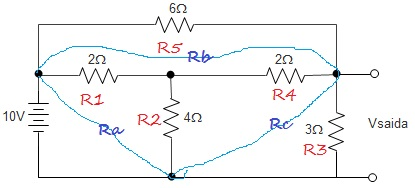
\includegraphics[scale=0.6]{fig1}
\caption{}
\label {f1}
\end{figure}\\
Convers\~ao $Y \longrightarrow\bigtriangleup$\\
\begin{eqnarray}
R_a=\frac{R_1R_2+R_2R_4+R_1R_4}{R_4}=10\Omega\\
R_c=10\Omega\\
R_b=5\Omega
\end{eqnarray}
\textit{- Vendo as que est\~ao em s\'erie e em paralelo sucede que: $R_t=3.34\Omega$}.\\
- \textit{A tens\~ao de sa\'ida \'e igual \`a queda de tens\~ao no resitor 3 e, \'e  $V_s=4.59V$}.
\vspace{4cm}
\item Determine a resistência de entrada equivalente entre os terminais a e d da fig.\ref{f2} sendo $R_1=10\Omega; R_2=8\Omega;R_3=2\Omega;R_4=2\Omega; $ e $R_5=10\Omega$.
\begin{figure}[htb]
\centering
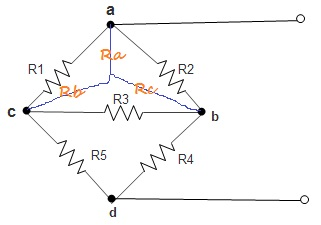
\includegraphics[scale=0.6]{fig2}
\caption{}
\label {f2}
\end{figure}

\it{Convers\~ao: $\bigtriangleup \longrightarrow Y$}\\
\begin{equation}
R_c=\frac{R_2 \times R_3}{R_1+R_2+R_3}
\end{equation}
 Repare que cada resist\^encia ser\'a o quociente entre o produto das duas resist\^encias adjacentes dividido pela soma de todas as que formam a rede triangular. Neste caso, para $R_c$, as duas resist\^encias adjacentes s\~ao $R_2$ e $R_3$.\\
\color{red}Assim: $R_t=5.16\Omega$ \color{black}
\rm
\item Determine a tensão de saída Vo do circuito da fig.\ref{fig3} sendo $R_1=30\Omega; R_2=10\Omega;R_3=5\Omega;R_4=10\Omega;R_5=10\Omega; $ e $R_6=30\Omega$.
 \begin{figure}[htb]
\centering
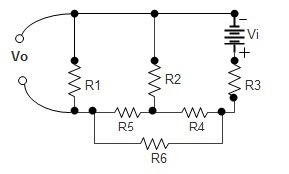
\includegraphics[scale=0.6]{fig3}
\caption{}
\label{fig3}
\end{figure}

\item Determine a condutância e a resistência total do circuito da fig.\ref{fig4} sendo $R_1=10\Omega; R_2=4\Omega;R_3=8\Omega$ e $R_4=2\Omega$.\\
i)	Usando a regra de divisor de corrente, determine a corrente que atravessa o resistor R3.
 \begin{figure}[htb]
\centering
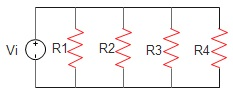
\includegraphics[scale=0.8]{fig4}
\caption{}
\label{fig4}
\end{figure}

\item Dado o circuito da fig.5  determine: i) o equivalente Thevenin e a queda de tensão na resistência de carga; ii) a queda de tensão na resistência de carga usando o princípio de sobreposição; iii) a queda de tensão na resistência de carga usando o teorema de Norton.

\end{enumerate}






\end{document}